\chapter{Diseño}

\section{Diseño de la arquitectura}
\label{sec:arquitectura}
La arquitectura de este sistema se basa en un modelo \textbf{cliente-base de datos}, donde el usuario interactúa únicamente con 
la interfaz gráfica de la aplicación (cliente), la cual se comunica con la base de datos \textit{Firebase Firestore} para obtener y almacenar la información. 
La interfaz gráfica se interactua directamente con la base de datos, sin necesidad de un servidor intermedio. Esta estructura simplifica el
desarrolo, al delegar en Firebase la gestión de la base de datos y la sincronización en tiempo real.

\subsection{Componentes Principales}

\begin{itemize}
    \item \textbf{Interfaz gráfica:} La interfaz gráfica es la parte de la aplicación con la que el usuario interactúa. 
    En este caso, la interfaz gráfica se ha diseñado para ser intuitiva y fácil de usar, con el objetivo de que el usuario pueda 
    realizar las tareas de forma rápida y sencilla.
    \item \textbf{Base de datos:} La base de datos es el componente encargado de almacenar y gestionar la información de la aplicación. 
    En este caso, se ha utilizado Firebase Firestore como base de datos, ya que permite almacenar y sincronizar los datos en tiempo real, 
    lo que facilita la gestión de la información.
\end{itemize}

\subsection{Flujo de interacción}

\begin{enumerate}
    \item El usuario accede a la aplicación y realiza una acción.
    \item La interfaz gráfica procesa la acción y envía la solicitud a la base de datos a través de las funciones de Firebase.
    \item La base de datos recibe la solicitud, la procesa y devuelve la información necesaria
    \item La interfaz gráfica recibe la información y la muestra al usuario.
\end{enumerate}


\section{Diseño de la interfaz gráfica}
\label{sec:interfaz}
El objetivo principal es conseguir la usabilidad de la aplicación, ya que aunque la aplicaciónn esté dirigida a un público joven, 
es importante que sea fácil de usar para cualquier usuario. Para ello, se va a diseñar una interfaz gráfica con un diseño sencillo 
teniendo en cuenta los siguientes críterios para que una aplicación sea usable:

\begin{itemize}
    \item \textbf{Simplicidad:} El diseño debe ser sencillo , evitando elementos innecesarios que puedan confundir al usuario.
    \item \textbf{Tamaño de los elementos:} Los elementos de la interfaz gráfica deben tener un tamaño adecuado para que el usuario pueda interactuar con ellos de forma cómoda.
    \item \textbf{Contraste:} Los colores y la tipografía deben tener un contraste adecuado para que el usuario pueda leer la información de forma clara.
    \item \textbf{Facilidad de navegación:} La interfaz gráfica debe ser fácil de navegar, permitiendo al usuario moverse de una pantalla a otra de forma rápida y sencilla.
\end{itemize}
    
\subsection{Interfaces de gráficas del Grupo 1: \textit{Gestión de sesión}}

En esta sección podemos ver todos los diseños de las interfaces gráficas del Grupo 1: \textit{Gestión de sesión}.

\begin{figure}[ht]
    \centering
    \begin{minipage}{0.45\textwidth}
        \centering
        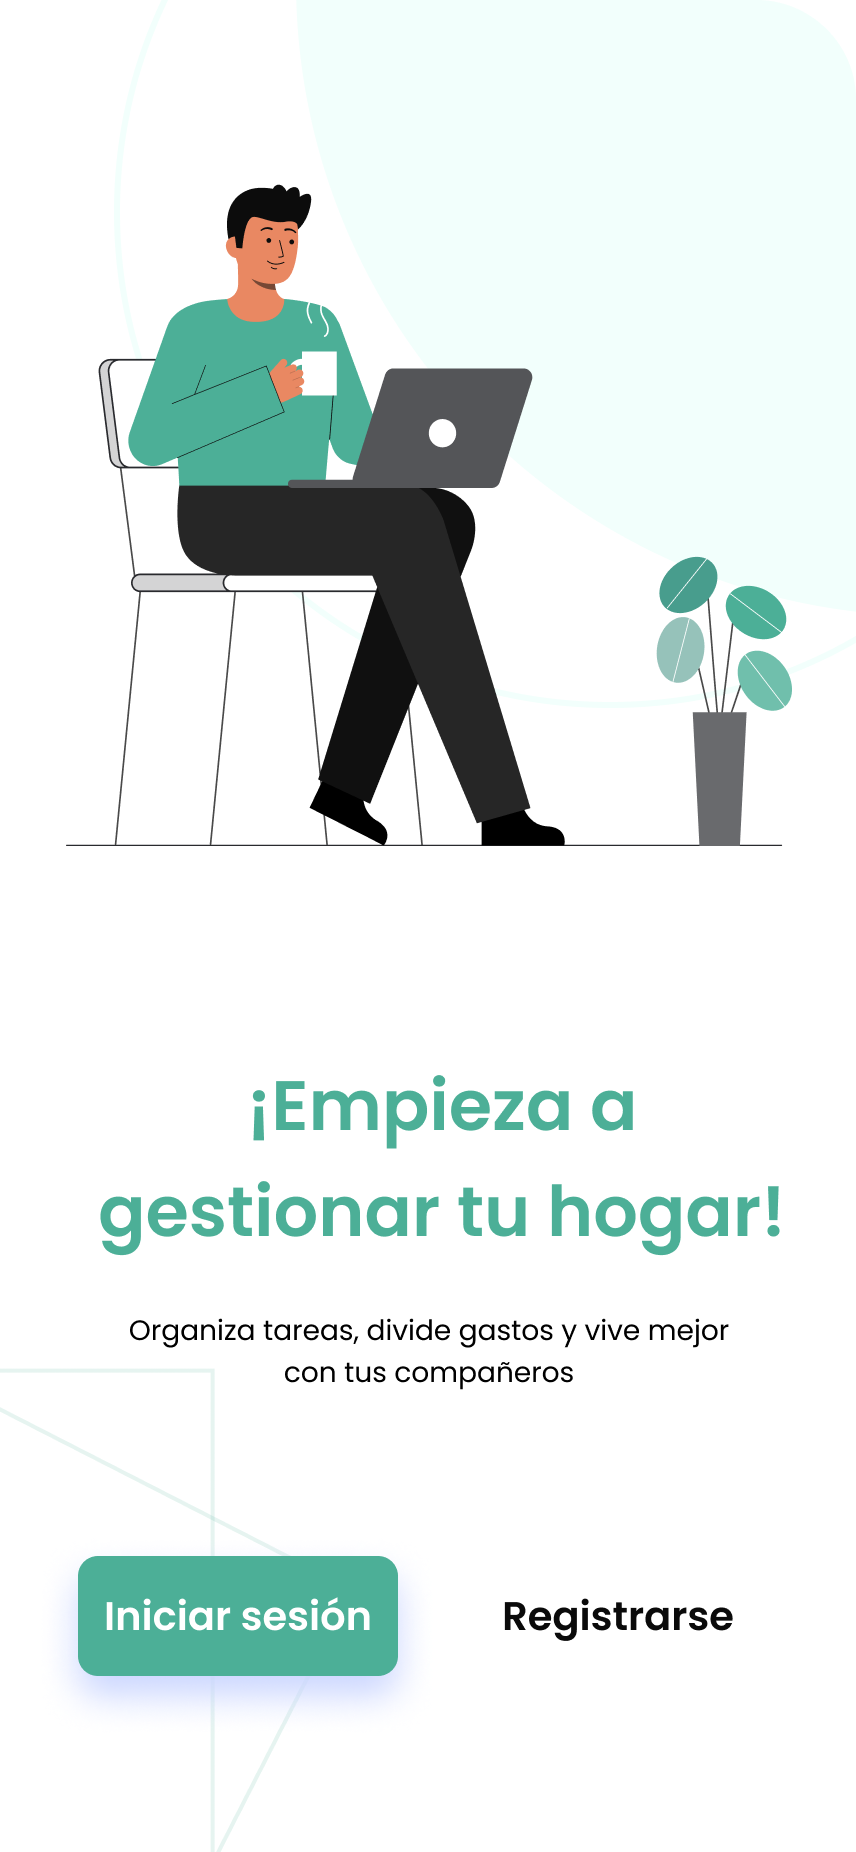
\includegraphics[width=\textwidth]{../capitulos/img/welcome_screen.png}
        \caption{Diseño de la pantalla de bienvenida.}
        \label{welcome}
    \end{minipage}
    \hfill
    \begin{minipage}{0.45\textwidth}
        \centering
        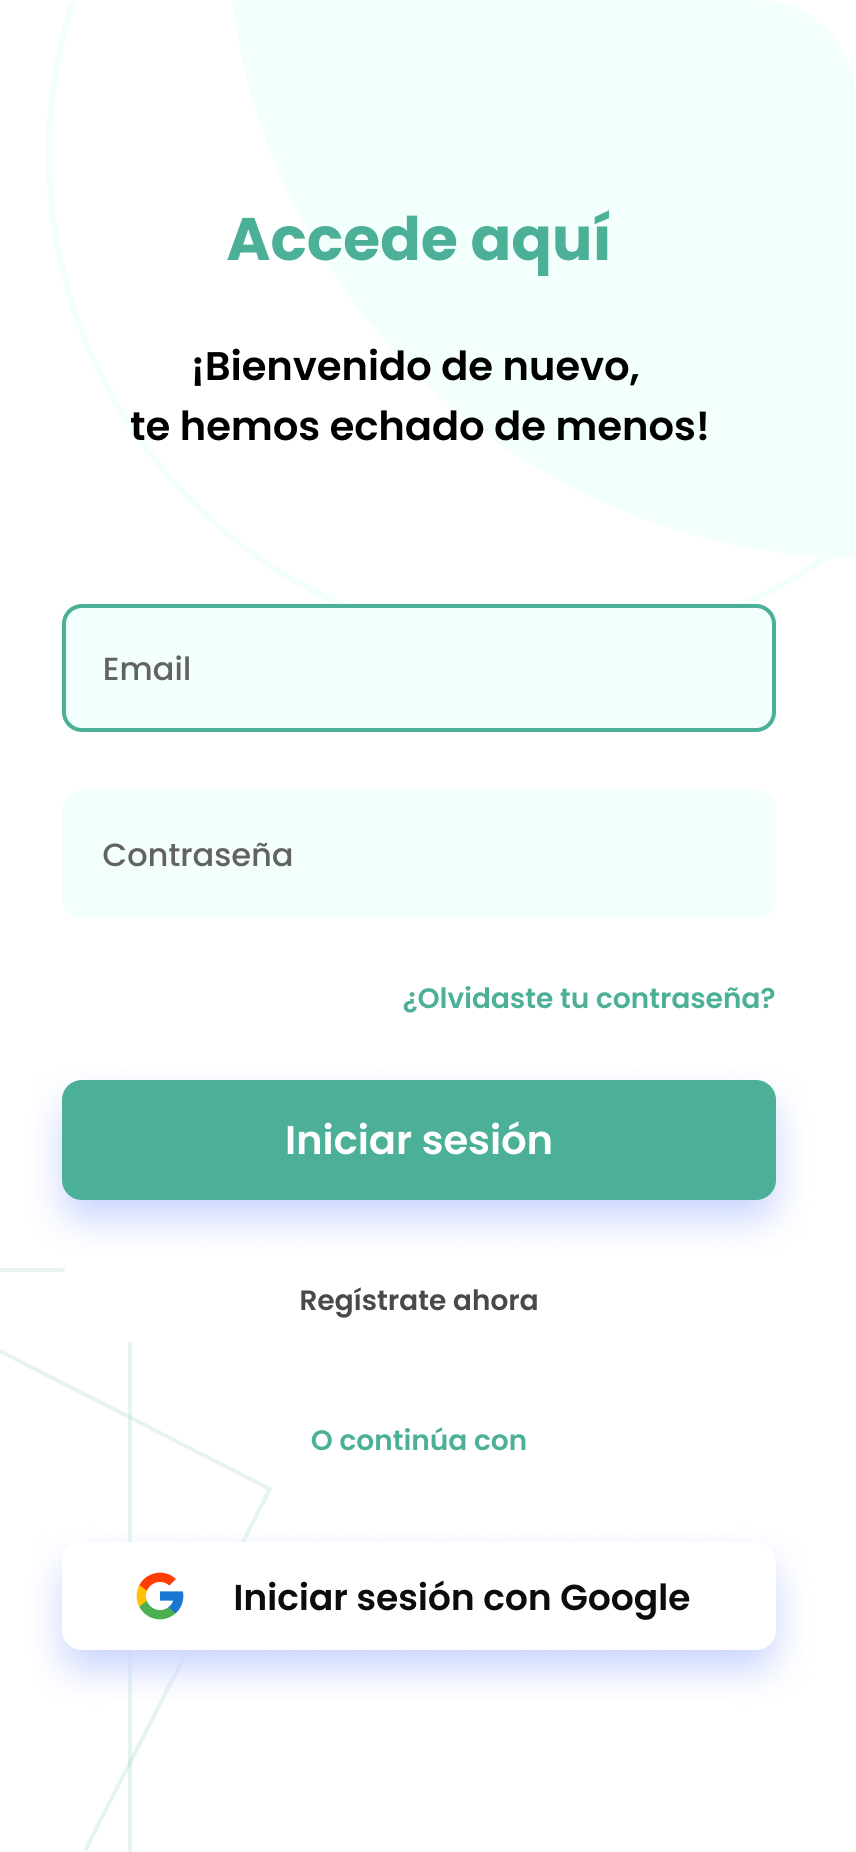
\includegraphics[width=\textwidth]{../capitulos/img/login_screen.png}
        \caption{Diseño de la pantalla de inicio de sesión.}
        \label{login}
    \end{minipage}
\end{figure}


\begin{figure}[ht]
    \centering
    \begin{minipage}{0.45\textwidth}
        \centering
        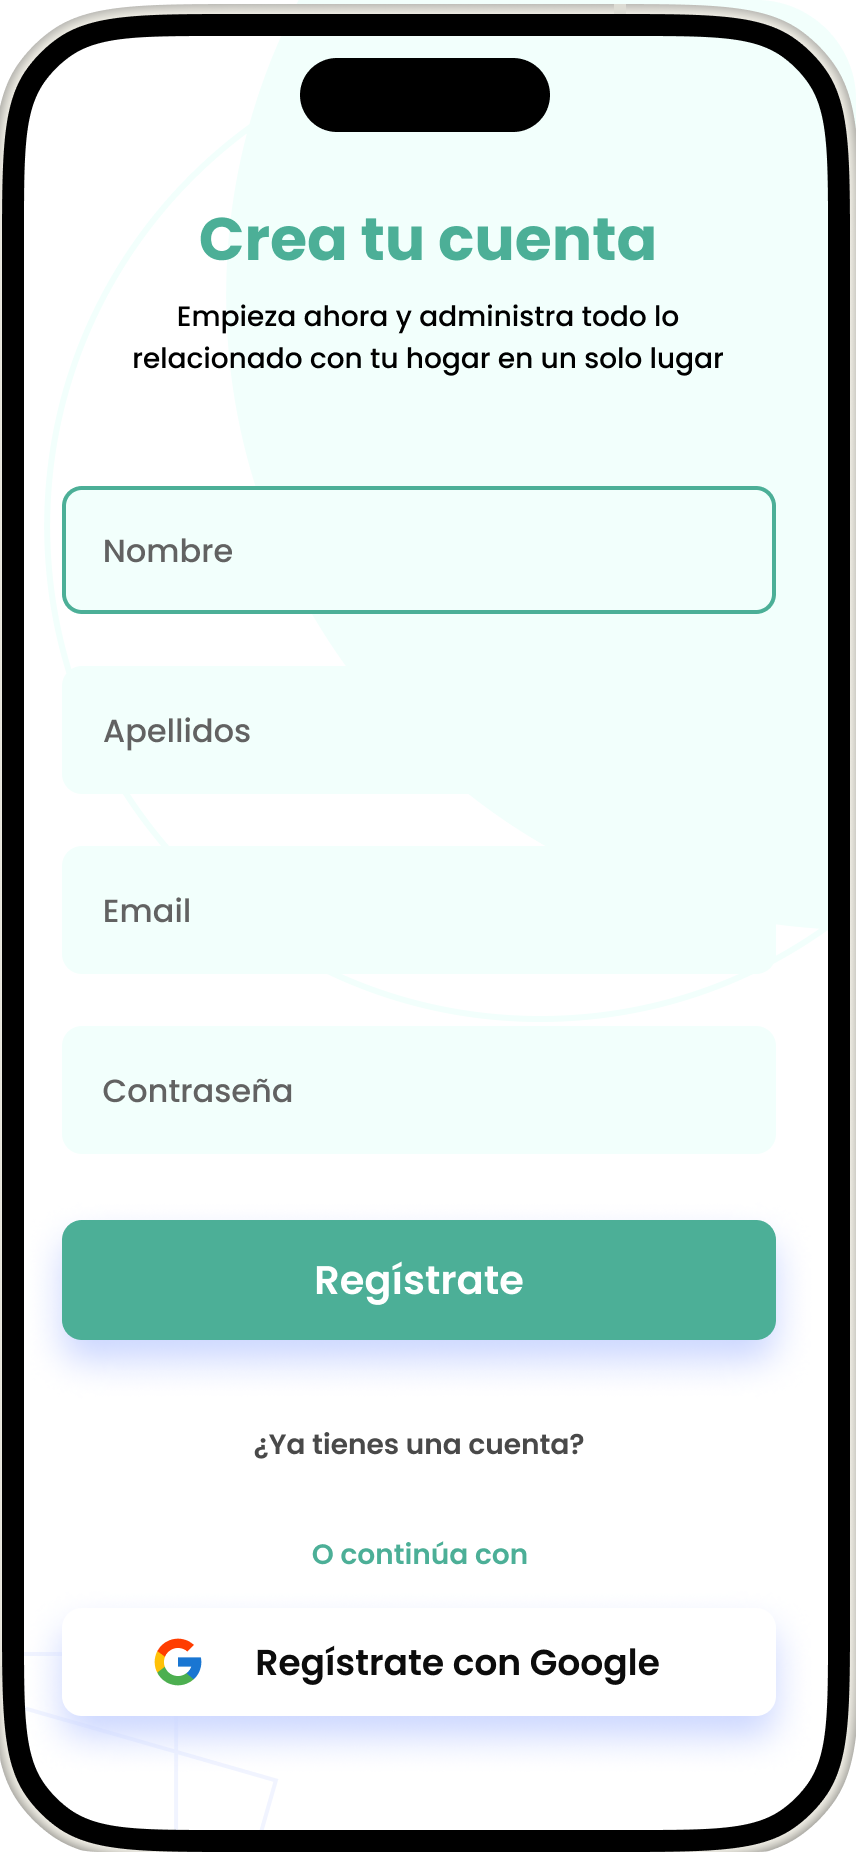
\includegraphics[width=\textwidth]{../capitulos/img/registro_screen.png}
        \caption{Diseño de la pantalla de registro.}
        \label{registro_app}
    \end{minipage}
    \hfill
    \begin{minipage}{0.45\textwidth}
        \centering
        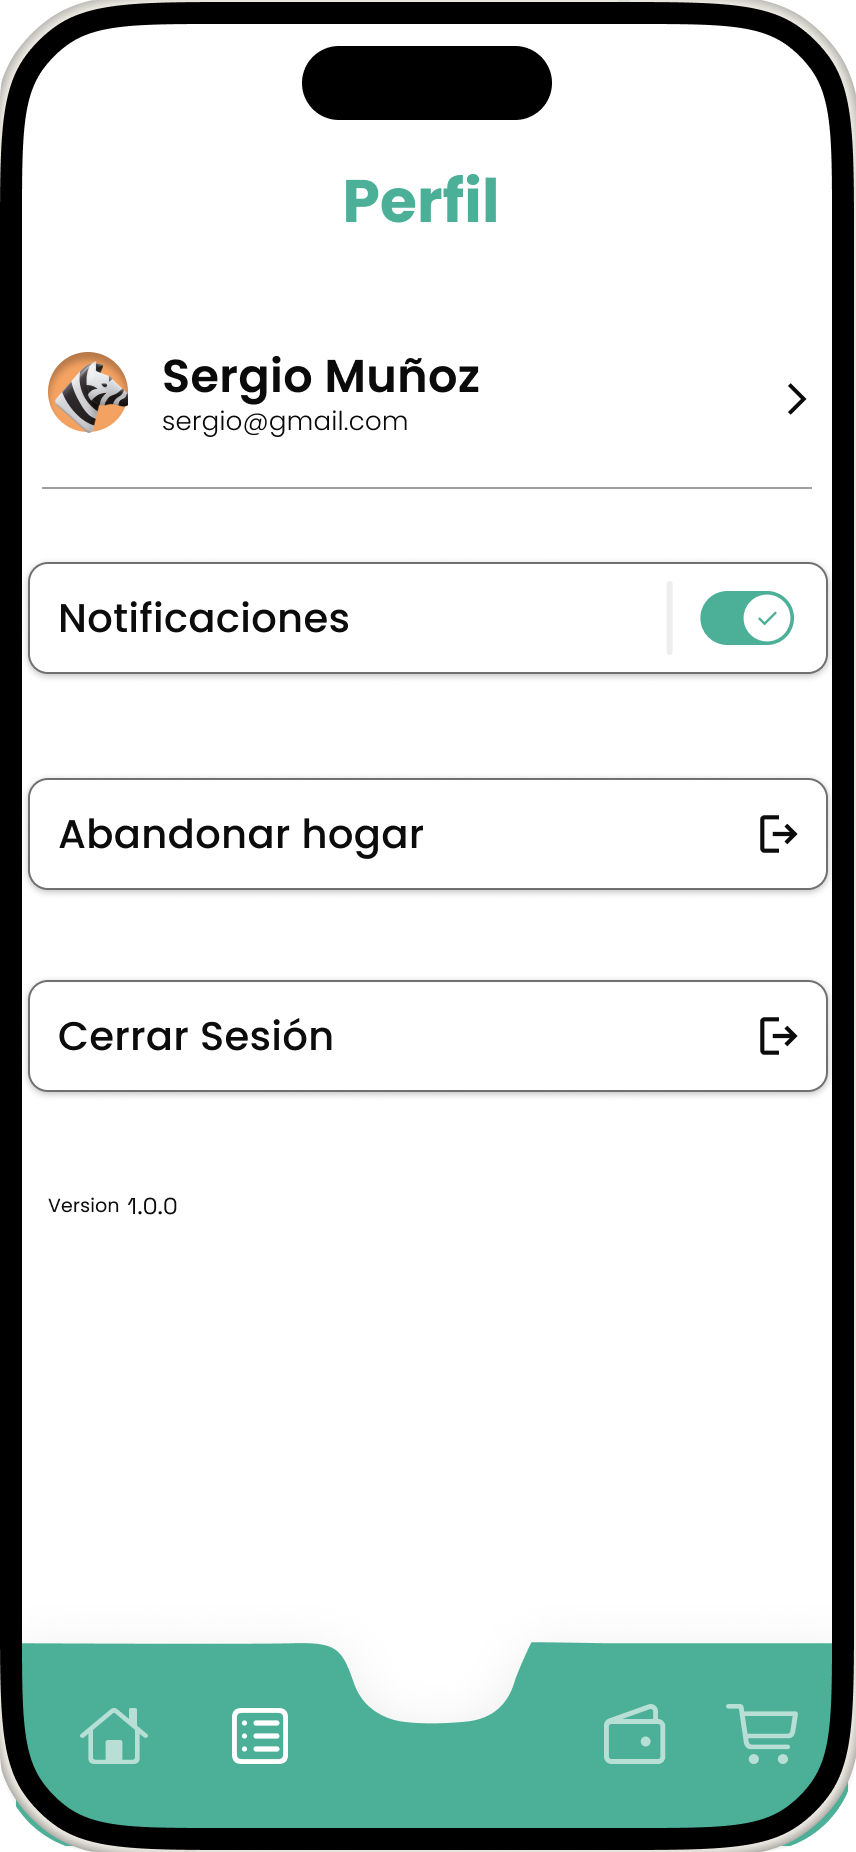
\includegraphics[width=\textwidth]{../capitulos/img/profile_screen.png}
        \caption{Diseño de la pantalla de cierre de sesión y datos de usuario.}
        \label{cierre}
    \end{minipage}
\end{figure}

\begin{figure}[ht]
    \centering
    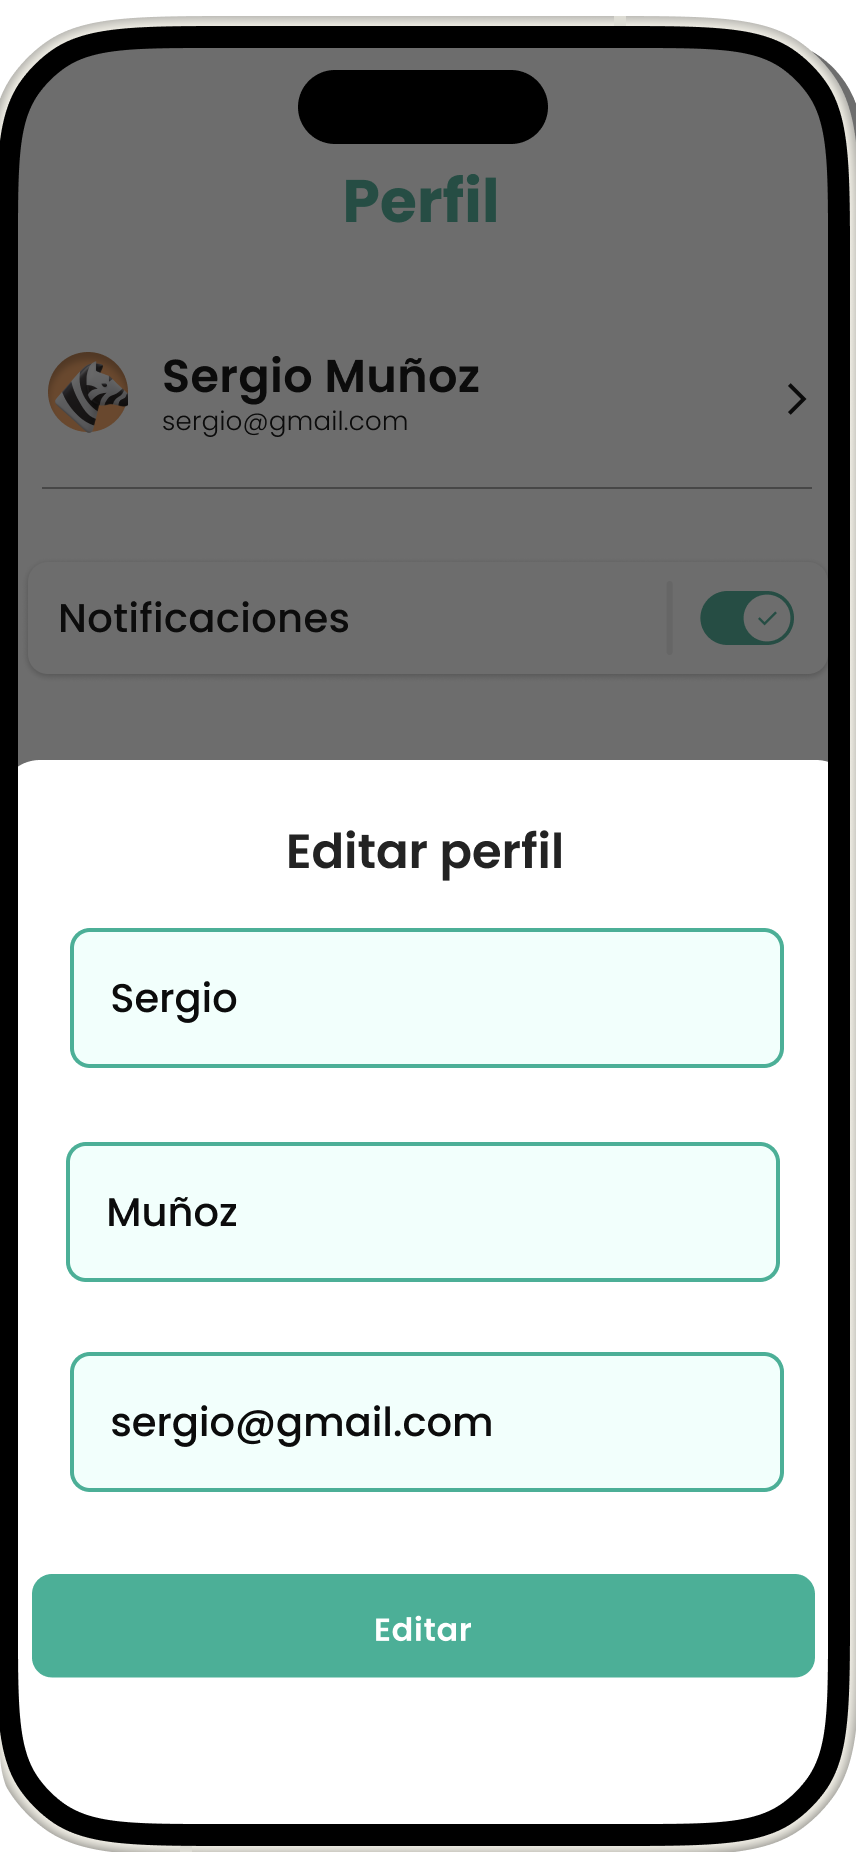
\includegraphics[width=0.45\textwidth]{../capitulos/img/edit_profile_screen.png}
    \caption{Diseño de la pantalla de editar perfil.}
    \label{edit_profile}
\end{figure}

\clearpage

\subsection{Interfaces de gráficas del Grupo 2: \textit{Gestión del hogar}}

\begin{figure}[ht]
    \centering
    \begin{minipage}{0.45\textwidth}
        \centering
        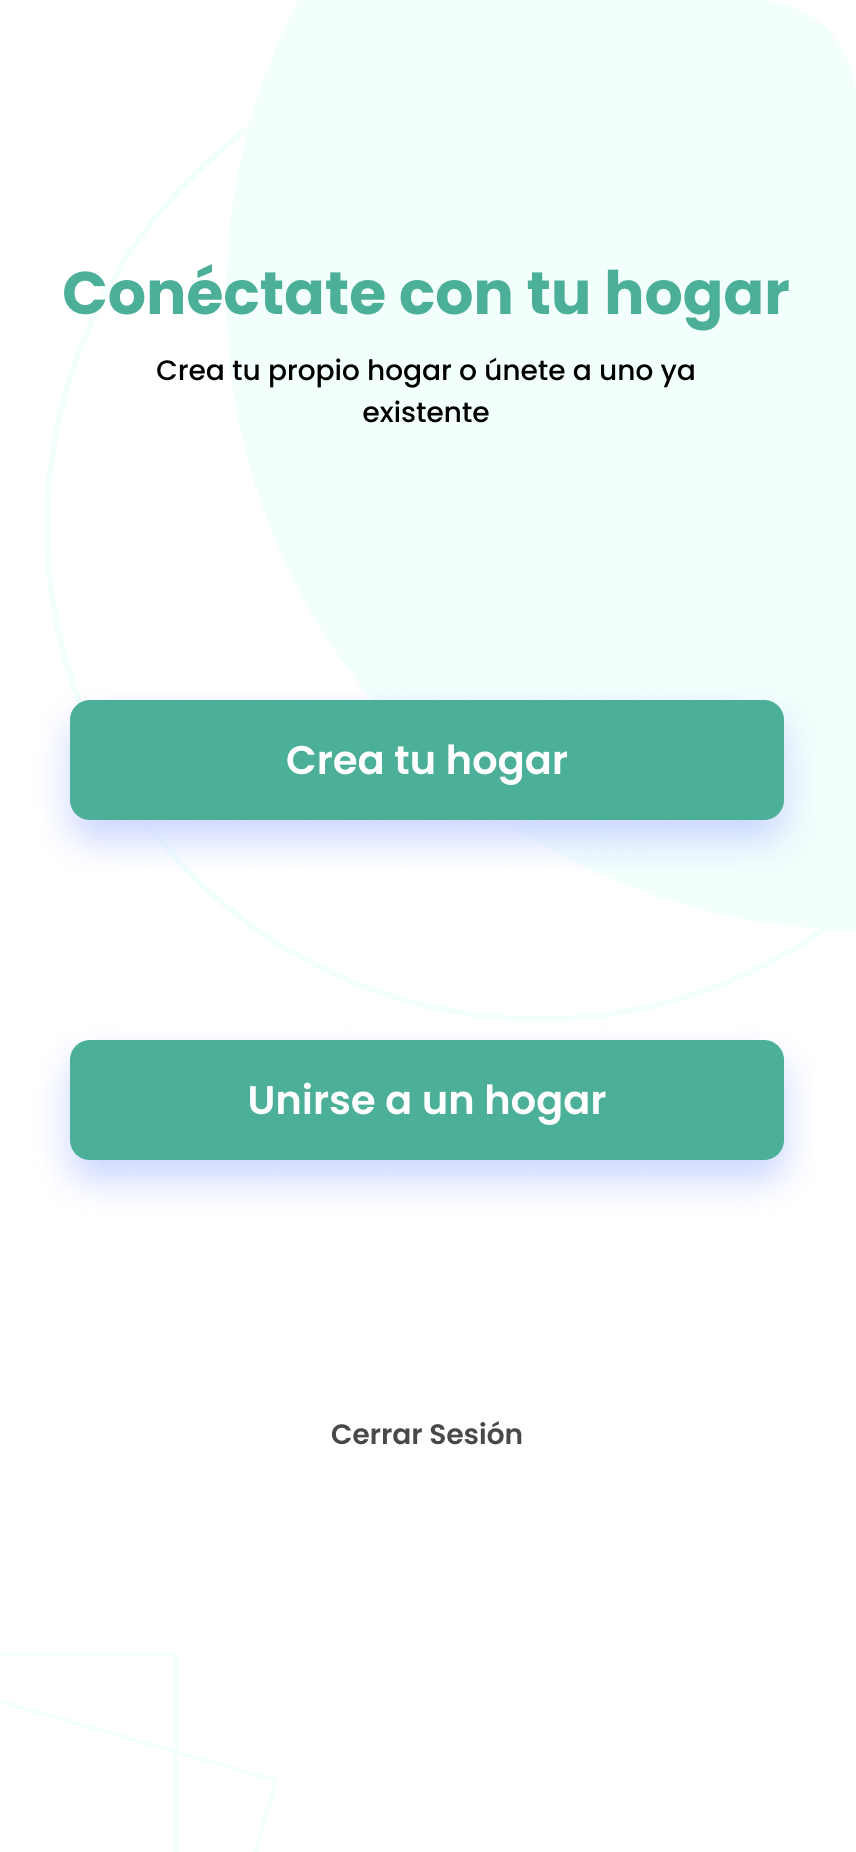
\includegraphics[width=\textwidth]{../capitulos/img/conect_screen.png}
        \caption{Diseño de la pantalla para unirte a un hogar o crear uno nuevo.}
        \label{conect}
    \end{minipage}
    \hfill
    \begin{minipage}{0.45\textwidth}
        \centering
        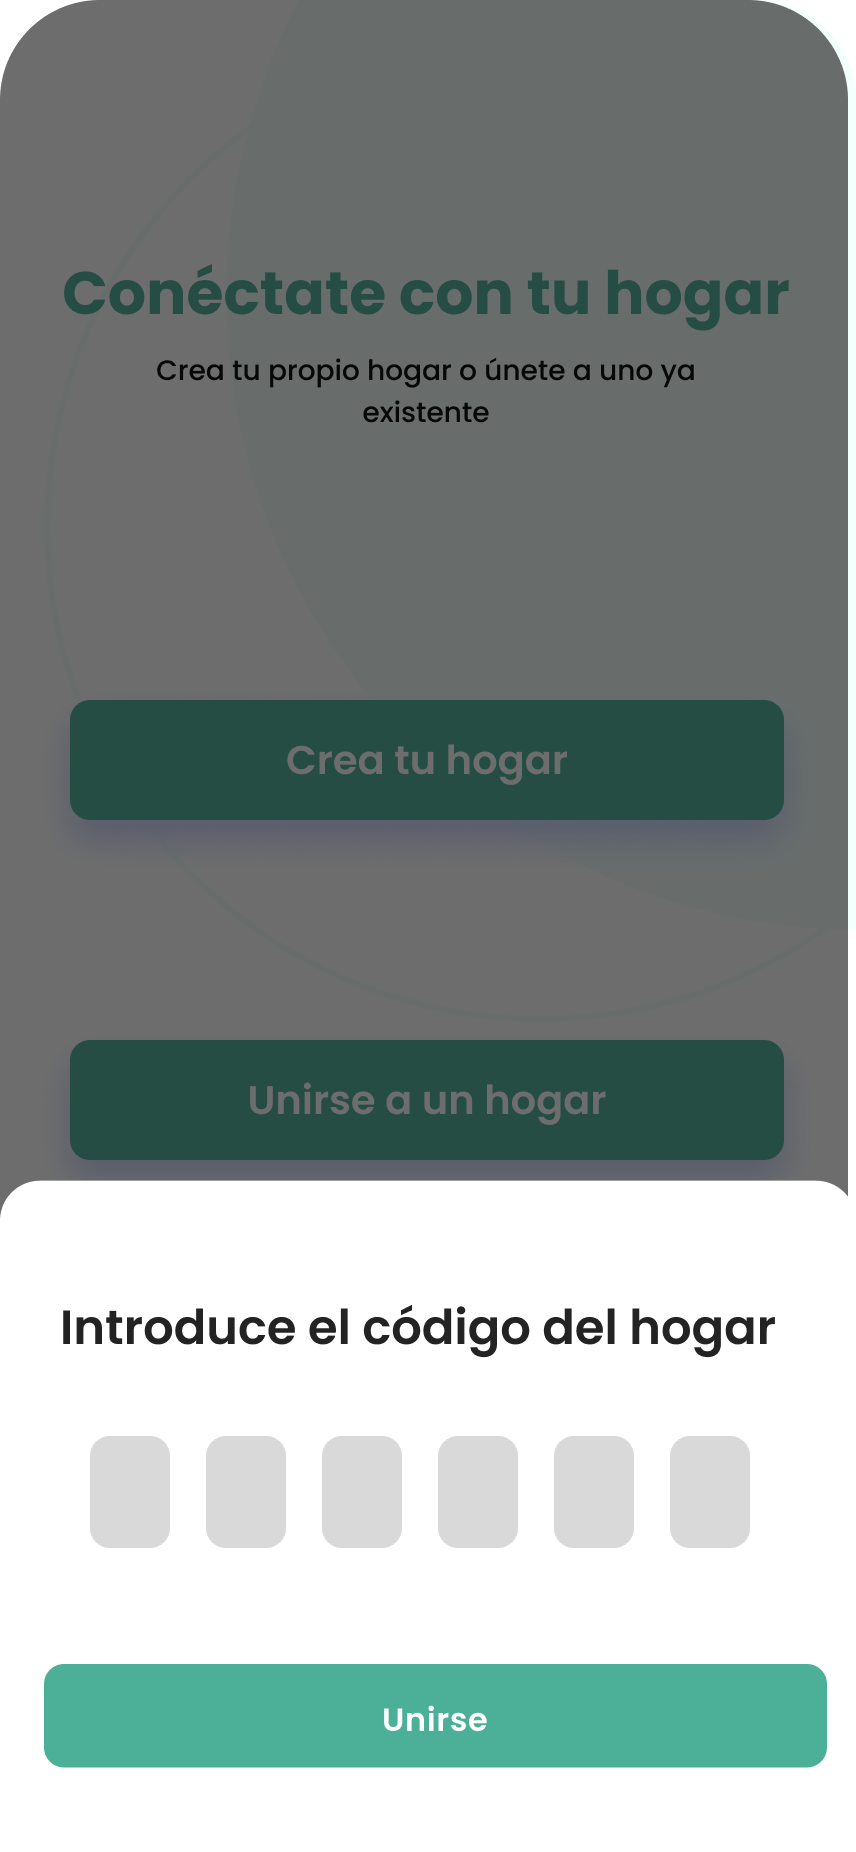
\includegraphics[width=\textwidth]{../capitulos/img/join_screen.png}
        \caption{Diseño de la pantalla para unirte a un hogar.}
        \label{join}
    \end{minipage}
\end{figure}

\begin{figure}[ht]
    \centering
    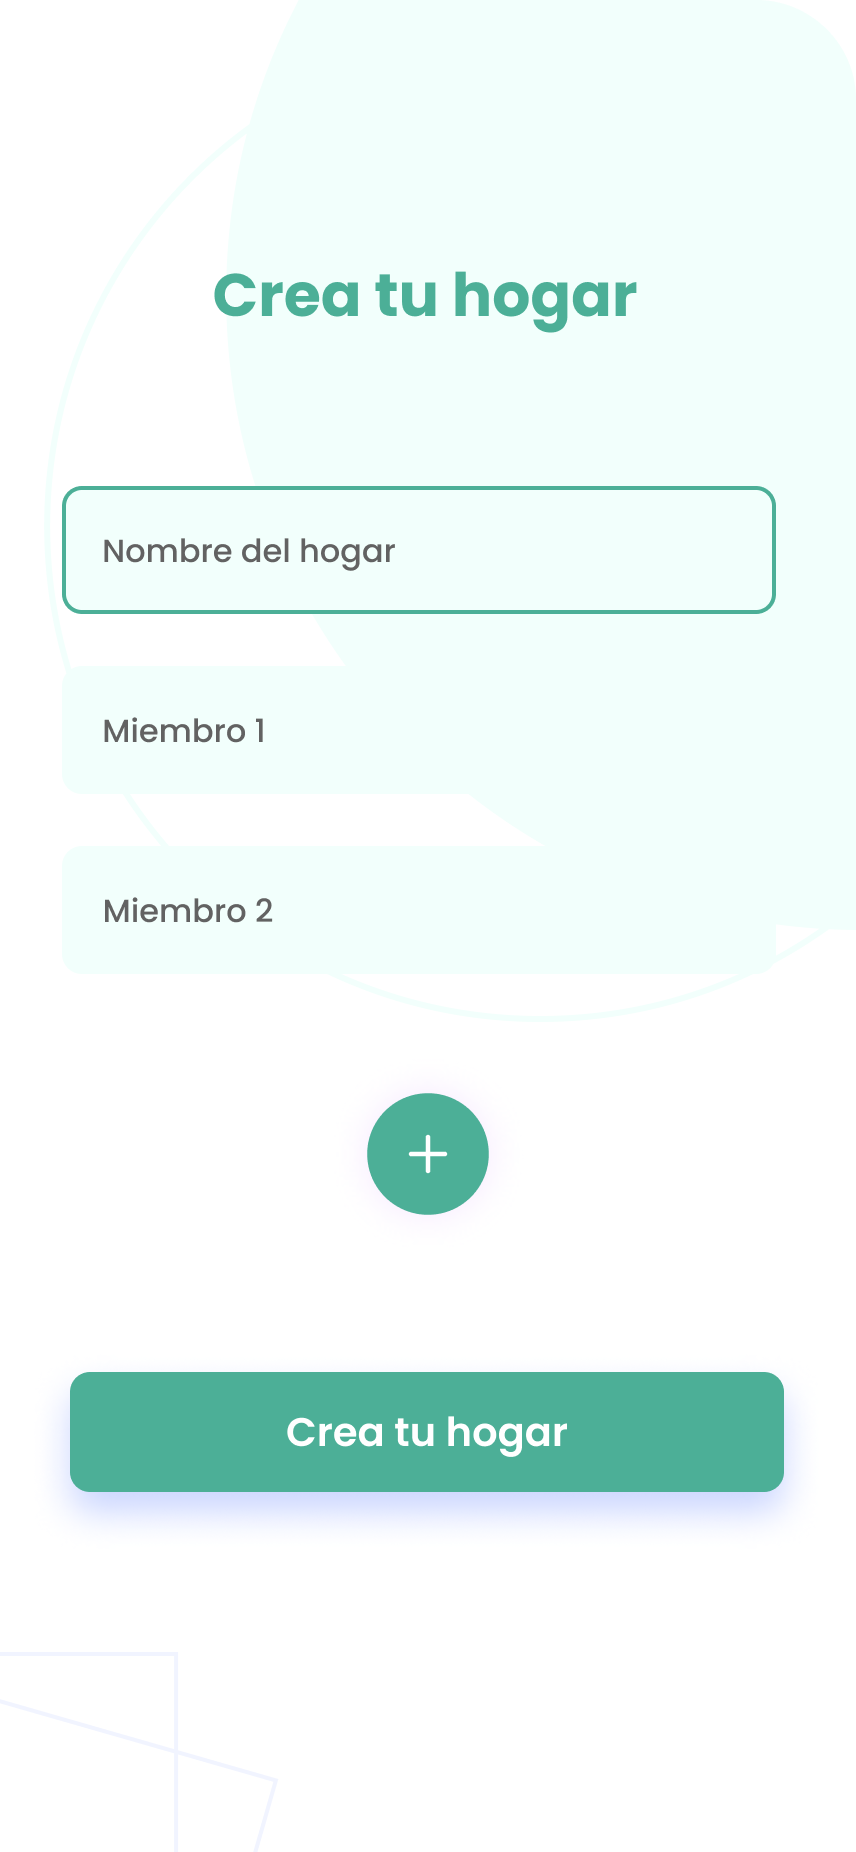
\includegraphics[width=0.45\textwidth]{../capitulos/img/new_home_screen.png}
    \caption{Diseño de la pantalla para crear un nuevo hogar.}
    \label{create_home}
\end{figure}



\clearpage

\subsection{Interfaces de gráficas del Grupo 3: \textit{Gestión de tareas}}

\begin{figure}[ht]
    \centering
    \begin{minipage}{0.45\textwidth}
        \centering
        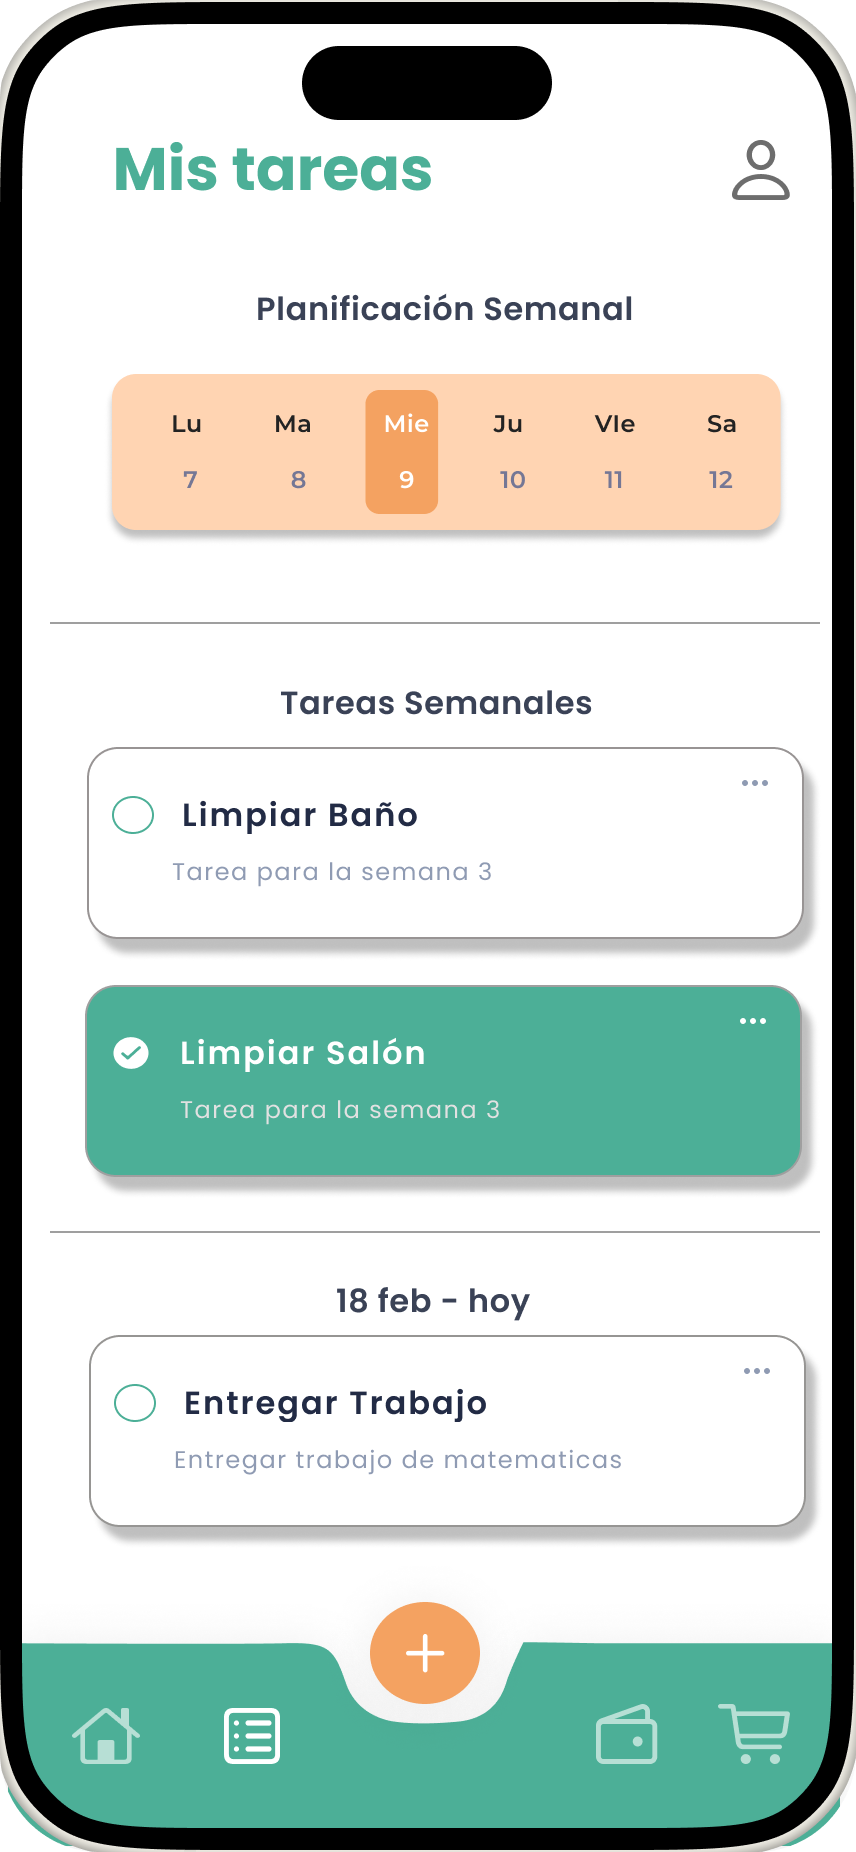
\includegraphics[width=\textwidth]{../capitulos/img/task_screen.png}
        \caption{Diseño de la pantalla principal de tareas.}
        \label{taks}
    \end{minipage}
    \hfill
    \begin{minipage}{0.45\textwidth}
        \centering
        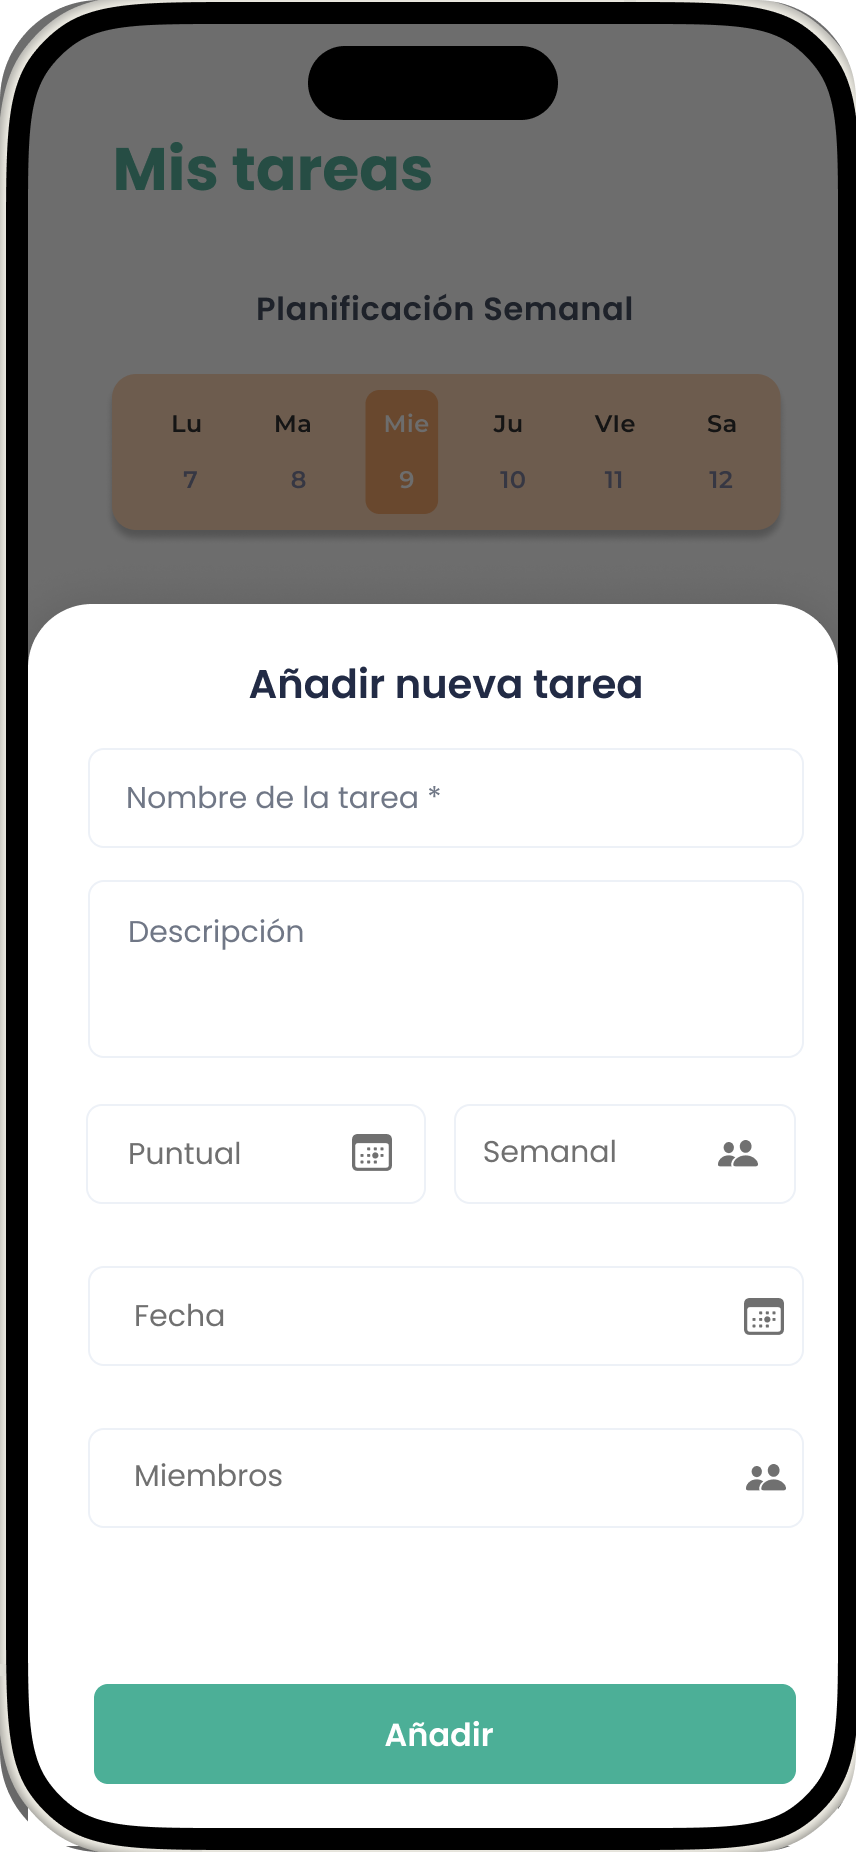
\includegraphics[width=\textwidth]{../capitulos/img/add_tasks_screen.png}
        \caption{Diseño de la pantalla para añadir una tarea.}
        \label{add_task}
    \end{minipage}
\end{figure}

\begin{figure}[ht]
    \centering
    \begin{minipage}{0.45\textwidth}
        \centering
        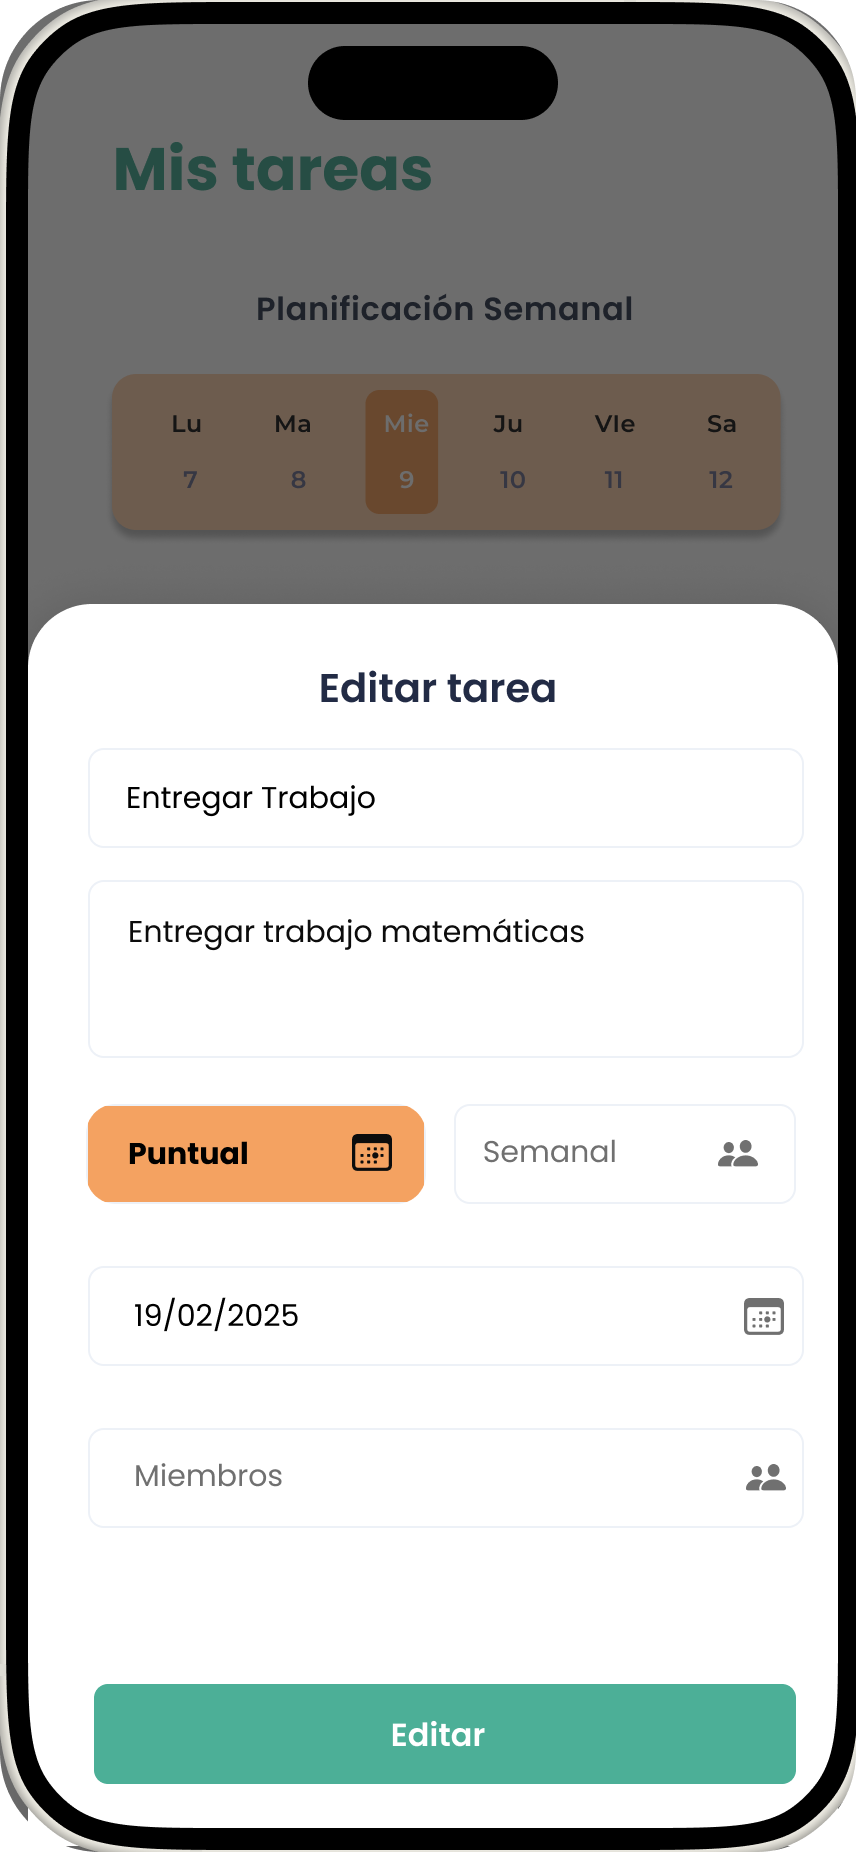
\includegraphics[width=\textwidth]{../capitulos/img/edit_task.png}
        \caption{Diseño de la pantalla para editar una tarea.}
        \label{edit_task}
    \end{minipage}
    \hfill
    \begin{minipage}{0.45\textwidth}
        \centering
        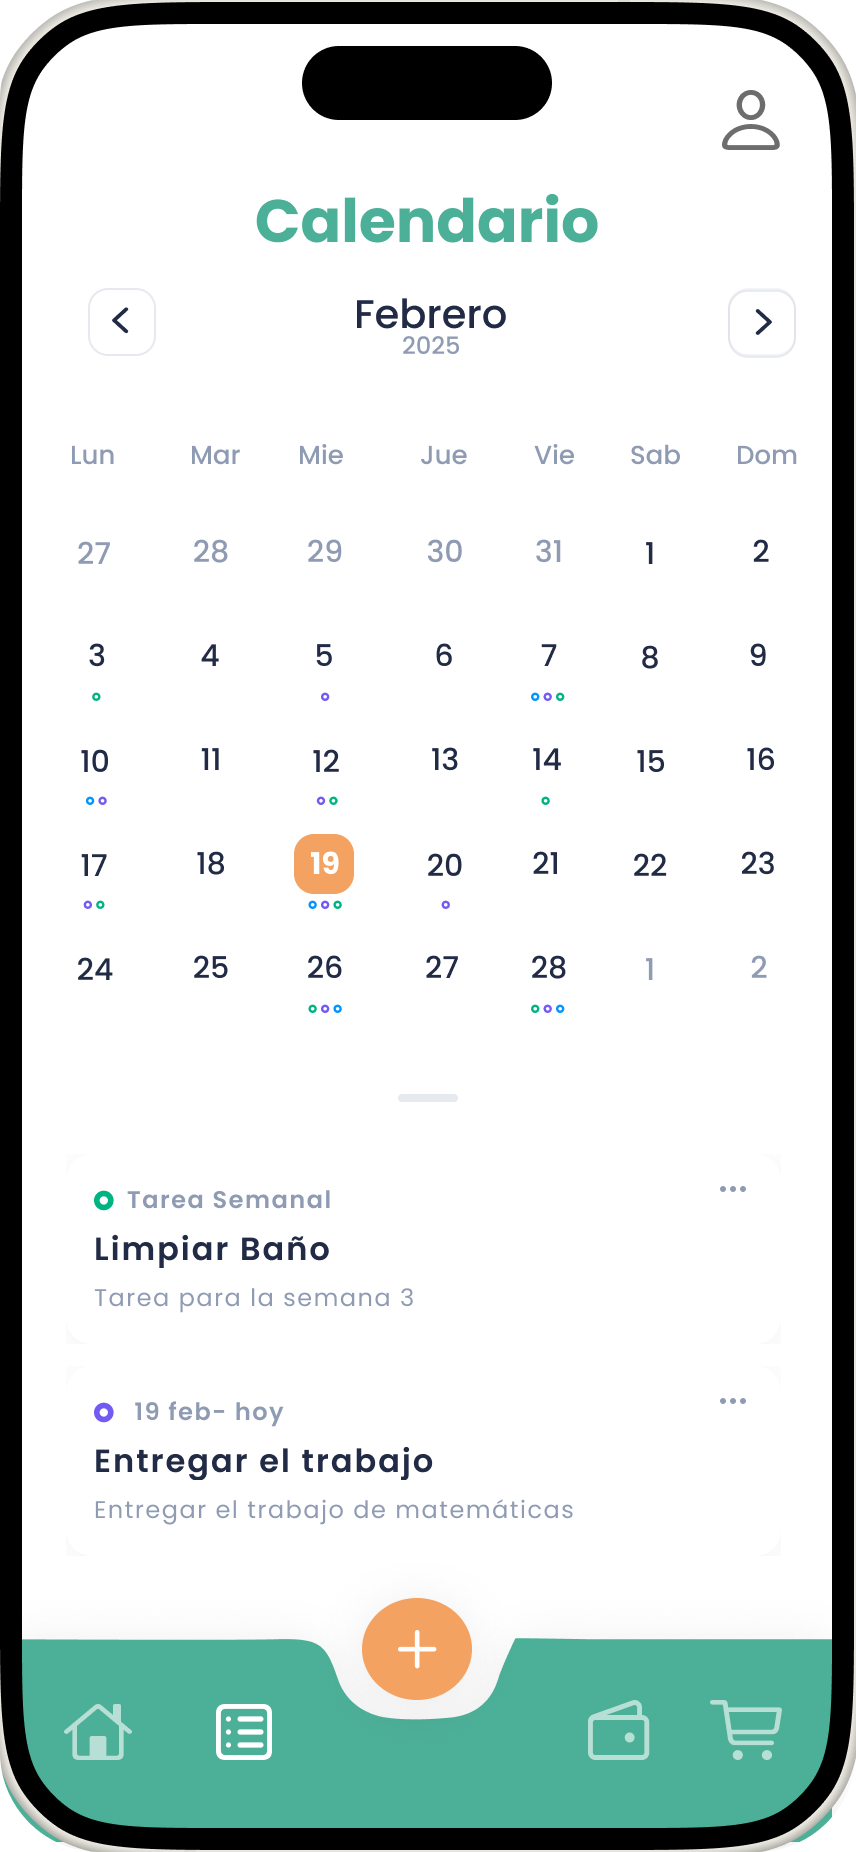
\includegraphics[width=\textwidth]{../capitulos/img/calendar_screen.png}
        \caption{Diseño de la pantalla del calendario.}
        \label{calendar}
    \end{minipage}
\end{figure}


\clearpage

\subsection{Interfaces de gráficas del Grupo 4: \textit{Gestión de gastos}}

\begin{figure}[ht]
    \centering
    \begin{minipage}{0.45\textwidth}
        \centering
        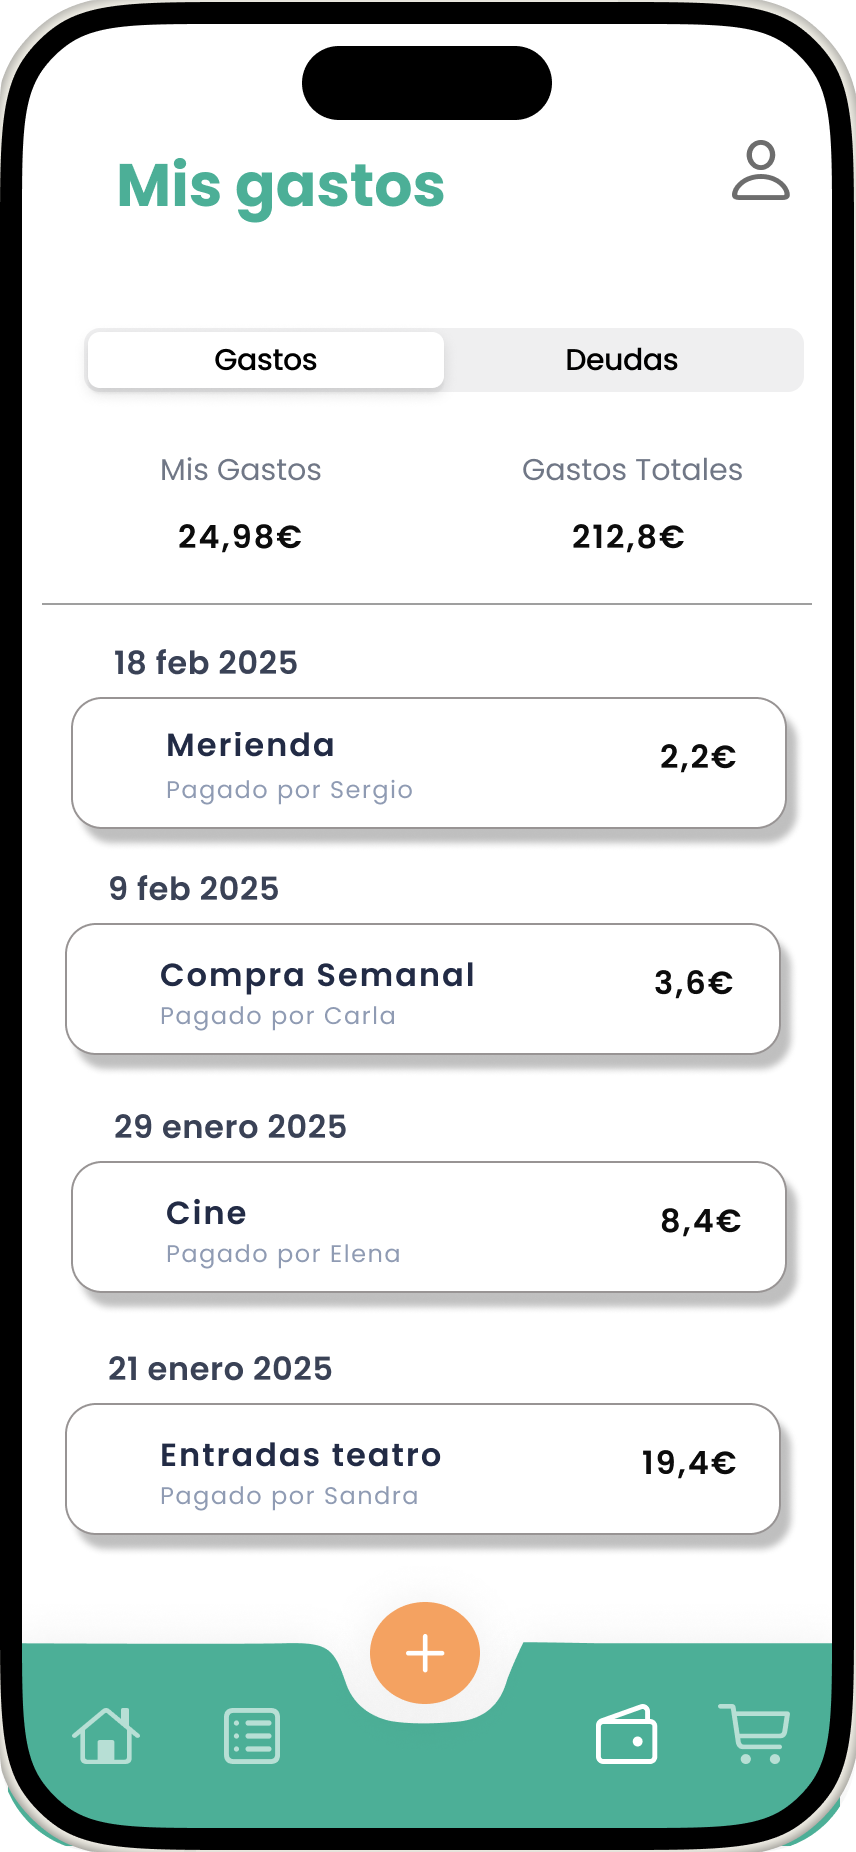
\includegraphics[width=\textwidth]{../capitulos/img/bills_screen.png}
        \caption{Diseño de la pantalla principal de gastos.}
        \label{expenses}
    \end{minipage}
    \hfill
    \begin{minipage}{0.45\textwidth}
        \centering
        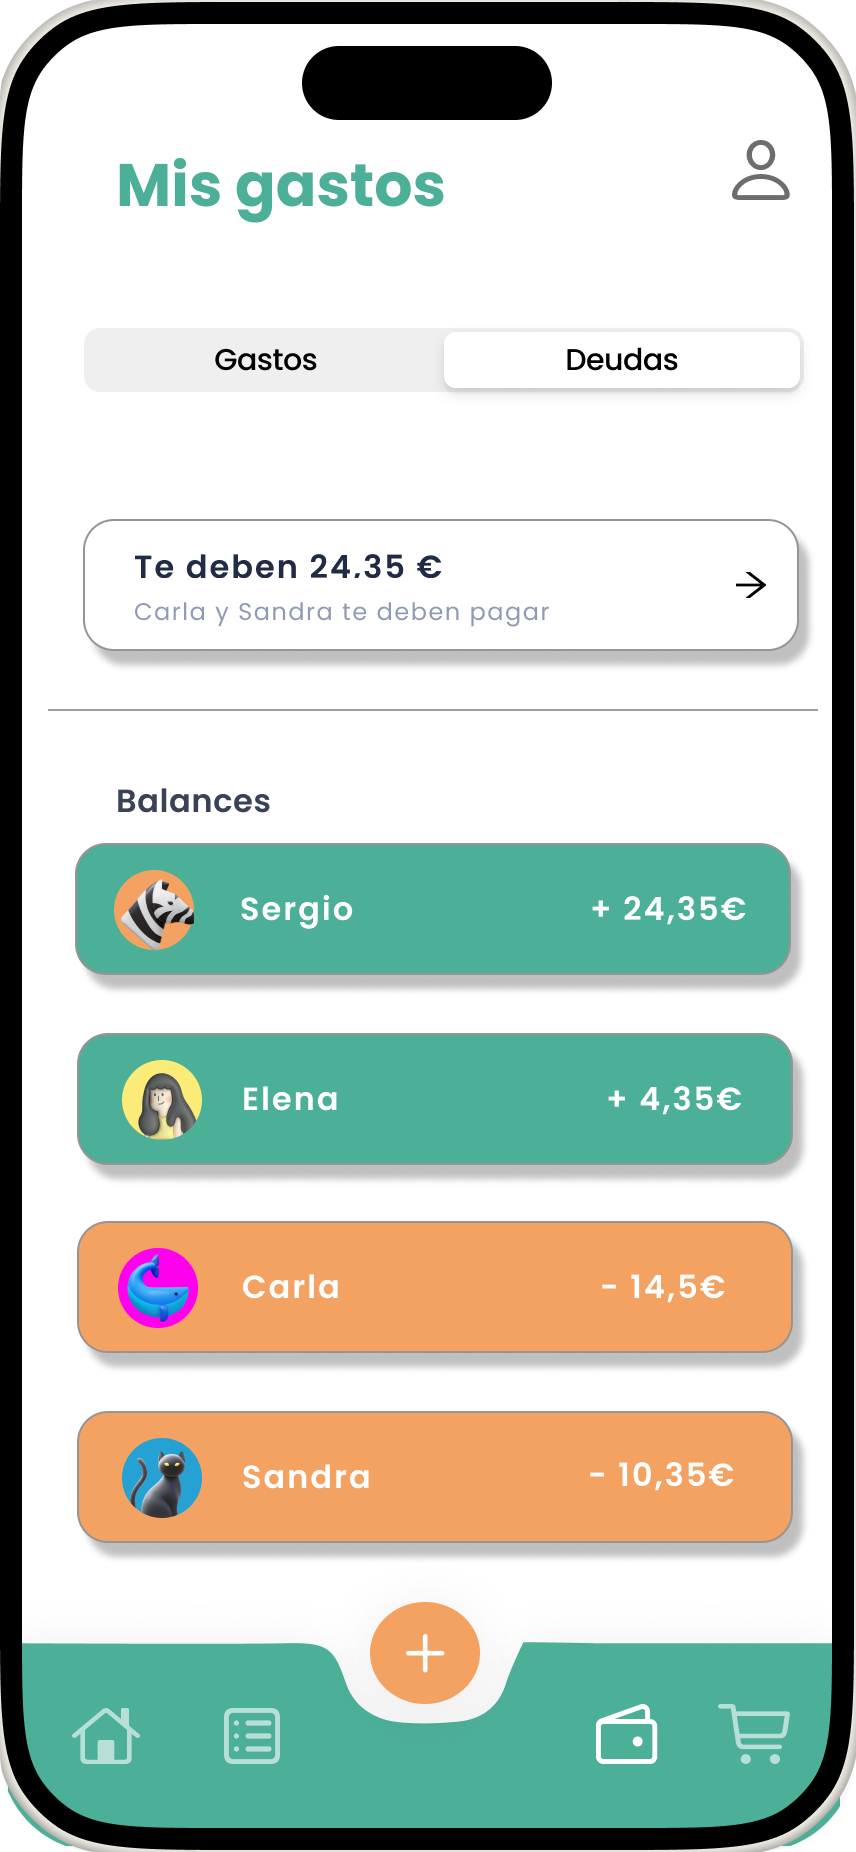
\includegraphics[width=\textwidth]{../capitulos/img/debs_screen.png}
        \caption{Diseño de la pantalla de deudas.}
        \label{debts}
    \end{minipage}
\end{figure}

\begin{figure}[ht]
    \centering
    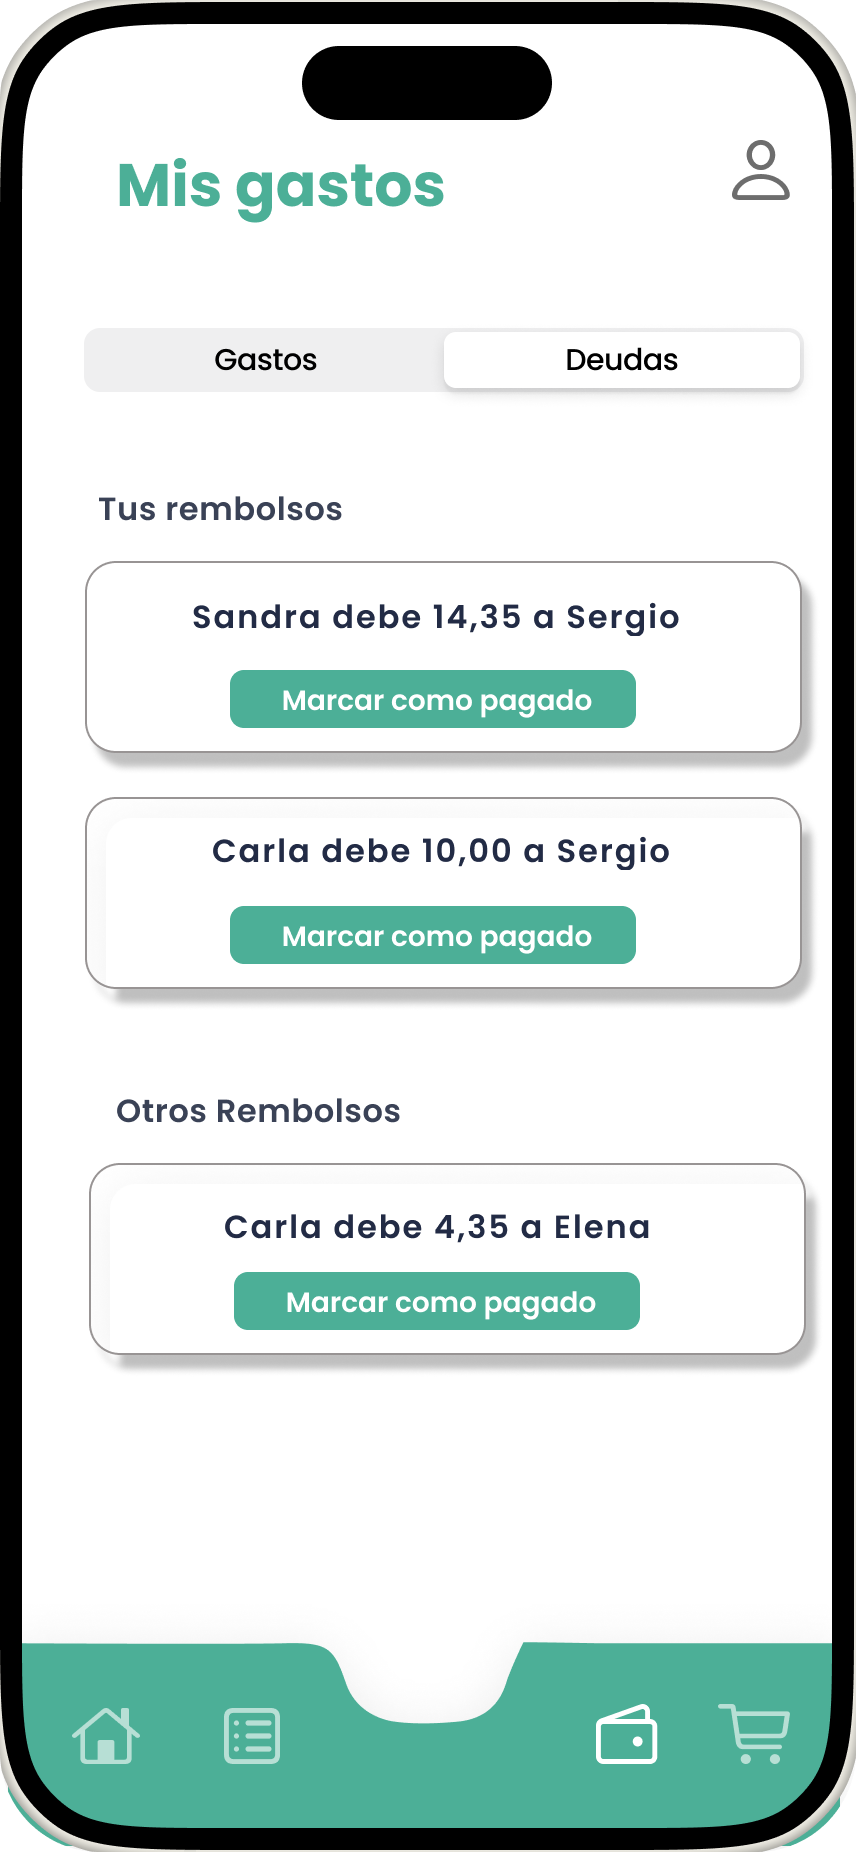
\includegraphics[width=0.45\textwidth]{../capitulos/img/pay_screen.png}
    \caption{Diseño de la pantalla para saldar deudas.}
    \label{settle_debts}
\end{figure}

\clearpage

\subsection{Interfaces de gráficas del Grupo 5: \textit{Gestión de la compra}}

\begin{figure}[ht]
    \centering
    \begin{minipage}{0.45\textwidth}
        \centering
        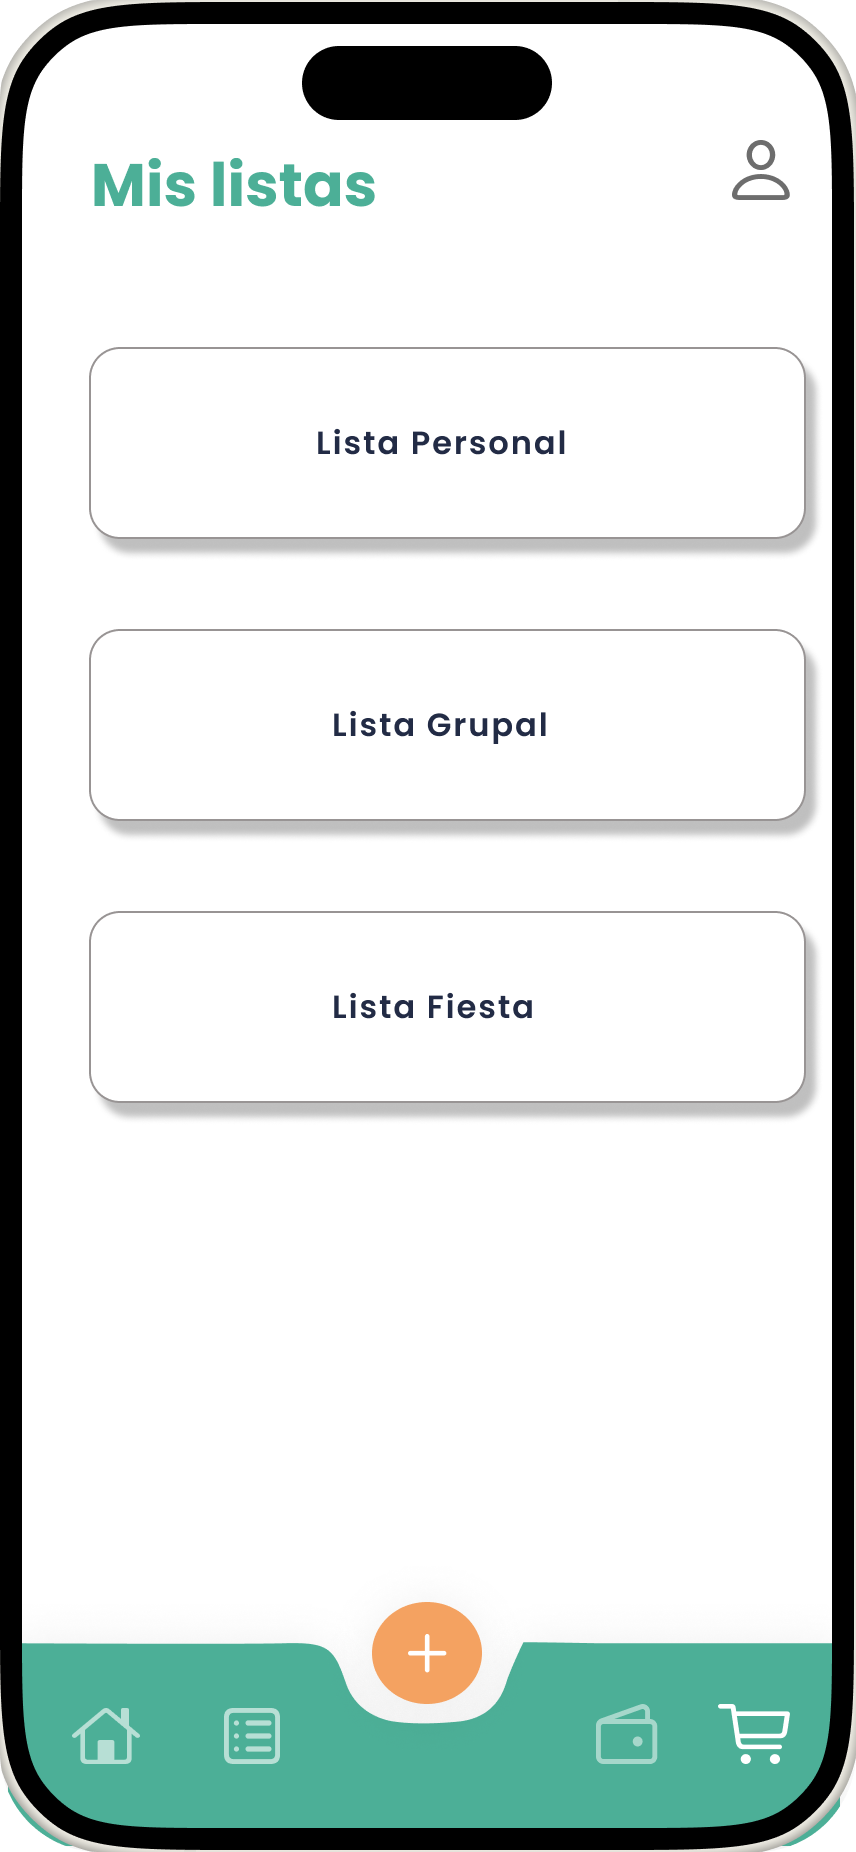
\includegraphics[width=\textwidth]{../capitulos/img/list_screen.png}
        \caption{Diseño de la pantalla de la lista de la compra.}
        \label{shopping_list}
    \end{minipage}
    \hfill
    \begin{minipage}{0.45\textwidth}
        \centering
        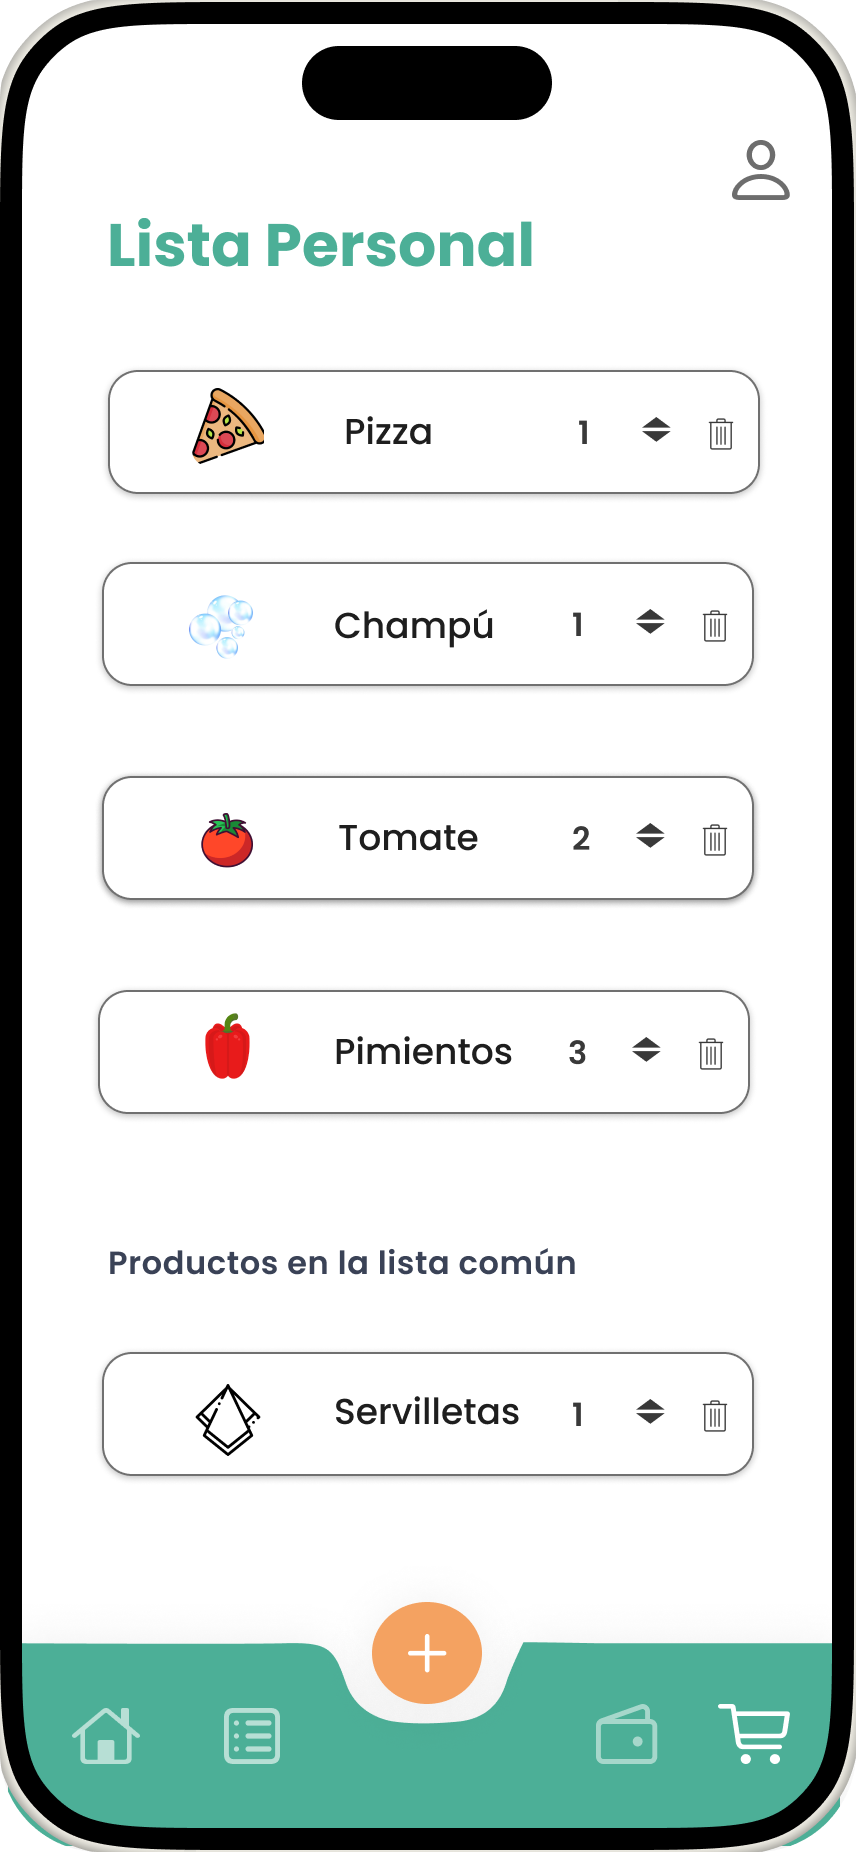
\includegraphics[width=\textwidth]{../capitulos/img/product_screen.png}
        \caption{Diseño de la pantalla de productos.}
        \label{products}
    \end{minipage}
\end{figure}

\newpage


